\chapter{Orbital-Free DFT}
The orbital-based formulation of density functional theory that was introduced by Kohn and Sham\cite{Kohn-Sham:1965} 
fifty years ago has been the most widely used method for determining the electronic structure 
of molecules during the last few decades. Even without the systematic improvability of the wave function based,
post-Hartree-Fock methods, modern density functional approximations are capable of reaching accuracies far
surpassing the Hartree-Fock method, but at similar computational cost, although some experience is required
for judging the applicability of each functional for a particular problem. 

Despite the tremendous success of the method, Kohn-Sham density functional theory (KS-DFT) still runs into 
trouble when applied to very large systems due to its relience on one-electron orbitals. For an $N$-electron
system, this leads to $N$ coupled, non-linear equations, for which a general solution scales approximately $N^3$,
although several order-$N$ methods have been proposed\cite{Goedecker:1999,Goedecker:2003,Watson:2004,Salek:2007}. 
Furthermore, in the limit of macroscopic 
systems, the notion of one-electron orbitals appears utterly impractical, and in fact, the 
Hohenberg-Kohn\cite{Hohenberg-Kohn:1964} theorems suggests that the key quantity should be the three-dimensional 
electron density, where the energy is given through the universal functional
\begin{equation}
    E[\rho] = T_s[\rho] + V_{en}[\rho] + J[\rho] + E_{xc}[\rho]
\end{equation}
In this expression we have kept the notion of non-interacting electrons that was introduced in Kohn-Sham theory,
and separated the energy into non-interacting kinetic energy $T_s$, classical electrostatic interaction between 
electrons and nuclei $V_{en}$ and between electrons $J$, and the quantum mechanical remainder $E_{xc}$, that 
accounts for electron exchange and correlation as well as the remaining "interacting" part of the kinetic energy.

\section{Density functionals}
In the early years of quantum mechanics, some futile attempts was made to model the kinetic and exchange energies
as pure density functionals. These models, by the work of Thomas\cite{Thomas:1927}, Fermi\cite{Fermi:1927} and 
Dirac\cite{Dirac:1929}, 
are based on theoretical considerations of the three-dimensional particle-in-a-box problem, and are exact for a 
non-interacting uniform electron gas. The Thomas-Fermi kinetic energy is given by
\begin{equation}
    \label{eq:thomas-fermi}
    T_{TF}[\rho] = \frac{3}{10}(3\pi^2)^{2/3} \int \rho^{5/3}(\bs{r}) \ud \bs{r}
\end{equation}
whereas the Dirac exchange energy has the form
\begin{equation}
    \label{eq:dirac}
    E_x[\rho] = -\frac{3}{4}\left(\frac{3}{\pi}\right)^{1/3} \int \rho^{4/3}(\bs{r}) \ud \bs{r}
\end{equation}
Needless to say, the uniform electron gas description does not apply to molecular densities, and the above
approximations (especially for the kinetic energy) fail to give even a qualitative description of real chemical 
systems (Teller\cite{Teller:1962} even proved that chemical binding is impossible within these models), and for this 
reason DFT was more or less discarded as a method for chemistry and solid-state physics. At that time, there was 
also no proof that the energy \emph{could} in fact be expressed as a functional of the electron density, 
and there was no theory of density functionals. 

This, of course, was going to change in the 1960's when a rigorous
theory was founded upon the Hohenberg-Kohn theorems, and practical (and accurate) calculations became available
through the Kohn-Sham formulation. Even so, the original orbital-free (OF-DFT) formulation was still regarded as
unsuited for treating molecular systems, mainly because of the many unsuccessful attempts of improving the accuracy 
of the kinetic energy functional.

However, some progress have been made over the years. The introduction of a gradient correction to the 
Thomas-Fermi energy by von Weiz\"{a}cker\cite{vonWeizacker:1935}
\begin{equation}
    \label{eq:vonWeizacker}
    T_W[\rho] = \frac{1}{8}\int\frac{|\nabla\rho(\bs{r})|^2}{\rho(\bs{r})}\ud\bs{r}
\end{equation}
which gives the exact energy for one- and two-electron (singlet) systems, made chemical binding possible. The more 
recent approaches are commonly separated into two distinct classes, one-point functionals
\begin{equation}
    T_s[\rho] = \int t_s(\rho;\bs{r})\ud\bs{r}
\end{equation}
and two-point functionals, which are able to reproduce the shell structure of atomic densities\cite{Wang:1992}
\begin{equation}
    T_s[\rho] = \int\int f_1(\rho;\bs{r})\chi(\bs{r},\bs{r}')f_2(\rho;\bs{r})\ud\bs{r}\ud\bs{r}'
\end{equation}
and a lot of work has gone into the development of new functionals based on purely theoretical 
considerations, see e.g. Karasiev \etal\cite{Karasiev:2009}. For 
instance, the exponents of the density appearing in the Thomas-Fermi and Dirac models are not arbitrary, but satisfy
the known coordinate scaling of the exact functional. A functional is said to be homogeneous of degree $m$ under
coordinate scaling if it satisfies
\begin{equation}
    F[\lambda^3\rho(\lambda\bs{r})] = \lambda^mF[\rho(\bs{r})]
\end{equation}
and the exact exchange and non-interacting kinetic energies are homogeneus of degree 1 and 2, respectively, leading 
to their respective exponents $\rho^{4/3}$ and $\rho^{5/3}$. 

In a recent work, Borgoo and Tozer\cite{Borgoo:2013} have looked
into the less familiar \emph{density scaling}, where a functional homogeneous of order $k$ satisfies
\begin{equation}
    F[\lambda\rho(\bs{r})] = \lambda^kF[\rho(\bs{r})]
\end{equation}
However, the sufficiently accurate approximation that would make OF-DFT useful for the description of molecular
systems remains to be found\cite{Xia:2012}, although some applications are found for large, periodic systems in 
condensed-phase physics in combination with pseudo-potentials, where the valence electrons are better 
approximated as a uniform electron gas\cite{Hung:2009,Huang:2010}.

Nevertheless, with the highly appealing prospect of fully realizing the Hohenberg-Kohn theorems by expressing
the energy purely as a functional of the density, work continues in finding better approximations. 

\section{Solution of the Euler equation}
In OF-DFT, the ground state density is obtained by solving a single three-dimensional Euler equation
\begin{equation}
    \label{eq:OF-Euler}
    \frac{\delta T_s[\rho]}{\delta \rho(\bs{r})} + v_{KS}(\bs{r}) = \mu
\end{equation}
where $v_{KS}$ is the effective potential of Kohn-Sham theory, as defined in Eq.~(\ref{eq:effective_pot}), and $\mu$ 
is the chemical potential. As the problem now involves the treatment of just a few global functions (density 
and potentials), instead of $N$ (possibly localized) one-electron orbitals appearing in KS-DFT, the lack of 
compactness of real-space representations becomes less of a problem\cite{Cervera:2006,Gavini:2006}. 
In particular, properties such as grid 
adaptivity and guaranteed accuracy should make the multiwavelet basis well suited to tackle the problem, if 
the equations can be formulated in such a way that an efficient optimization is possible. 

It is common to separate the non-interacting kinetic energy into the von Weiz\"{a}cker contribution given in
Eq.~(\ref{eq:vonWeizacker}) plus a non-negative remainder, known as the Pauli term
\begin{equation}
    T_s[\rho] = T_W[\rho] + T_\theta[\rho], \qquad T_\theta[\rho] \geq 0
\end{equation}
The functional derivative of the von Weiz\"{a}cker energy is
\begin{equation}
    \frac{\delta T_W[\rho]}{\delta \rho(\bs{r})} = 
	\frac{1}{\sqrt{\rho(\bs{r})}}\Big(-\frac{1}{2}\nabla^2\Big)\sqrt{\rho(\bs{r})}
\end{equation}
which brings the Euler equation over to the form
\begin{equation}
    \Big[-\frac{1}{2}\nabla^2 + v_\theta(\bs{r}) + v_{KS}(\bs{r})\Big]\sqrt{\rho(\bs{r})} =
	\mu\sqrt{\rho(\bs{r})} 
\end{equation}
which is identical to the Kohn-Sham equations for one "orbital" $\orbital(\bs{r}) = \sqrt{\rho(\bs{r})}$ 
and effective potential $v_{eff} = v_\theta + v_{nuc} + v_{el} + v_{xc}$
\begin{equation}
    \label{eq:OF-orbital}
    \Big[-\frac{1}{2}\nabla^2 + v_{eff}(\bs{r})\Big]\orbital(\bs{r}) = \mu\orbital(\bs{r})
\end{equation}
The similarity with the KS equations have lead to the misconception that the problem can be easily solved 
to self-consistency by any Kohn-Sham solver by only minor modifications\cite{Levy:1984}. More recent
studies, however, have shown the opposite, both in the context of the usual atomic GTOs\cite{Chan:2000}
and in a real-space numerical basis\cite{Karasiev:2012}. The claim is that the kinetic energy is to non-quadratic
for a straightforward iterative optimization, and that more robust techniques are required, like the one 
presented by Jiang \etal\cite{Jiang:2004}.

\section{Preliminary results}
In the following we will attempt to solve the OF-DFT Euler equation (\ref{eq:OF-Euler}) in the multiwavelet 
framework using a modified form of the KS-DFT solver that is presented in publication III. The iterative
procedure is based on the one-orbital formulation given in Eq.~(\ref{eq:OF-orbital}), and thus relies on the
von Weiz\"{a}cker kinetic energy functional. The singel orbital is normalized to the number of electrons 
$\langle\orbital|\orbital\rangle = N$, so that the density is given as
\begin{equation}
    \rho(\bs{r}) = |\orbital(\bs{r})|^2
\end{equation}
Also appearing in the equation is the usual nuclear and electronic potentials
\begin{align}
    v_{nuc}(\bs{r}) &= \sum_{I} \frac{Z_I}{\|\bs{r}-\bs{R}_I\|} \\
    v_{el}(\bs{r}) &= \int \frac{\rho(\bs{r}')}{\|\bs{r}-\bs{r}'\|} \ud\bs{r}'
\end{align}
where the singularities in the nuclear potential have been smoothed out as described in publication III, 
originally introduced by Harrison \etal\cite{Harrison:2004}. As $v_{xc}$ we choose the simple Dirac exchange
functional presented above in Eq.~(\ref{eq:dirac}) with no correlation treatment, which gives the potential
\begin{equation}
    v_{xc}(\bs{r}) = \frac{\delta E_x[\rho]}{\delta \rho} = -\left(\frac{3}{\pi}\right)^{1/3} \rho^{1/3}(\bs{r})
\end{equation}
and we perform calculations both in the Dirac-vonWeiz\"{a}cker (DvW) model, where the Pauli term is zero 
$T_\theta = 0$, and in the Thomas-Fermi-Dirac-vonWeiz\"{a}cker (TFDvW) model, where the Pauli term is chosen as
the Thomas-Fermi kinetic functional given in Eq.~(\ref{eq:thomas-fermi}), giving a purely repulsive potential
\begin{equation}
    v_\theta(\bs{r}) = \frac{\delta T_\theta[\rho]}{\delta\rho} = \frac{1}{2}\left(3\pi^2\right)^{2/3} \rho^{2/3}(\bs{r})
\end{equation}
The results (chemical potential and total energy) of such calculations are presented in table \ref{tab:of-results}, where
the total energies are compared to conventional (spin-restricted) KS-DFT calculations, using the same Dirac exchange,
as well as (spin-restricted) Hartree-Fock energies, taken from Karasiev and Trickey\cite{Karasiev:2012} and Chan 
\etal\cite{Chan:2000}, respectively (The Hartree-Fock energies presented in Ref.\cite{Chan:2000} are actually calculations 
taken from an old reference, Clementi and Roetti\cite{Clementi:1974}).

\begin{table}
\footnotesize
\begin{center}
\begin{tabular}{ll|ll|llll}
\hline
\hline
    &			    &\multicolumn{2}{|c|}{Chemical potential}&\multicolumn{4}{|c}{Total energy (Hartree)}\\
    &			    &
\multicolumn{1}{|c}{DvW}&
\multicolumn{1}{c|}{TFDvW}&
\multicolumn{1}{c}{DvW}&
\multicolumn{1}{c}{TFDvW}&
\multicolumn{1}{c}{LDA}&
\multicolumn{1}{c}{RHF}\\
\hline                                                      
H   & MRChem			&  -0.194320    &  -0.071640    &   -0.406534   &  -0.261826    &   -0.406534   &   -0.500000   \\
    & Ref.\cite{Chan:2000}	&	        &  -0.071	&		&  -0.2618      &	        &   -0.5000     \\
    & Ref.\cite{Karasiev:2012}  &  -0.1943      &  -0.0715      &   -0.406534   &  -0.261827    &   -0.4065     &	        \\
\hline                                                      
He  & MRChem			&  -0.516991    &  -0.108327    &   -2.723640   &  -1.477451    &	        &	        \\
    & Ref.\cite{Chan:2000}	&	        &  -0.108       &               &  -1.4775      &	        &   -2.8617     \\
    & Ref.\cite{Karasiev:2012}	&	        &               &               &               &   -2.7236     &	        \\
\hline                                                      
Li  & MRChem			&  -0.957510    &  -0.130656    &   -8.525825   &  -4.105425    &	        &		\\
    & Ref.\cite{Chan:2000}	&	        &  -0.131       &               &  -4.1054      &	        &   -7.4327	\\
    & Ref.\cite{Karasiev:2012}	&  -0.9575      &  -0.1306      &   -8.525825   &  -4.105425    &   -7.1749     &	        \\
\hline                                                      
Be  & MRChem			&  -1.510360    &  -0.145379    &  -19.352891   &  -8.492186    &	        &	        \\
    & Ref.\cite{Chan:2000}	&	        &  -0.145       &               &  -8.4922      &	        &  -14.5730     \\
    & Ref.\cite{Karasiev:2012}	&	        &               &               &               &  -14.2233     &	        \\
\hline                                                      
B   & MRChem			&  -2.172342    &  -0.155706    &  -36.729140   & -14.925883    &	        &	        \\
    & Ref.\cite{Chan:2000}	&	        &  -0.156       &               & -14.9258      &	        &  -24.5291     \\
    & Ref.\cite{Karasiev:2012}	&	        &               &               &               &  -24.5275     &	        \\
\hline                                                      
C   & MRChem			&  -2.941311    &  -0.163319    &  -62.169552   & -23.656875    &	        &	        \\
    & Ref.\cite{Chan:2000}	&	        &  -0.163       &               & -23.6568      &	        &  -37.6886     \\
    & Ref.\cite{Karasiev:2012}	&	        &               &               &               &  -37.6863     &	        \\
\hline                                                      
N   & MRChem			&  -3.815709    &  -0.169164    &  -97.182735   & -34.908435    &	        &	        \\
    & Ref.\cite{Chan:2000}	&	        &  -0.169       &               & -34.9084      &	        &  -54.4009     \\
    & Ref.\cite{Karasiev:2012}  &	        &               &               &               &  -54.3977     &	        \\
\hline                                                      
O   & MRChem			&  -4.794343    &  -0.173804    & -143.272616   & -48.883228    &	        &	        \\
    & Ref.\cite{Chan:2000}	&	        &  -0.174       &               & -48.8831      &	        &  -74.8094     \\
    & Ref.\cite{Karasiev:2012}  &		&               &               &               &  -74.8076     &	        \\
\hline                                                      
F   & MRChem			&  -5.876263    &  -0.177591    & -201.939506   & -65.767584    &	        &	        \\
    & Ref.\cite{Chan:2000}	&	        &  -0.178       &               & -65.7674      &	        &  -99.4094     \\
    & Ref.\cite{Karasiev:2012}  &	        &	        &               &               &  -99.4072     &	        \\
\hline                                                      
Ne  & MRChem			&  -7.060692    &  -0.180760    & -274.680827   & -85.734479    & -127.490748   & -128.547101   \\
    & Ref.\cite{Chan:2000}	&	        &  -0.181       &	        & -85.7343      &		& -128.5471     \\
    & Ref.\cite{Karasiev:2012}  &  -7.0607	&  -0.1807      & -274.68080    & -85.734451    & -127.4907	&	        \\
\hline                                                      
H$_2$	& MRChem		&  -0.331330    &  -0.100168    &   -1.043736   &  -0.430723    &   -1.043736   &   -1.133619   \\
BH	& MRChem		&  -1.170066    &  -0.146852    &  -38.589138   & -15.301851    &  -24.629804   &  -25.131640   \\
\hline                                                                                  
\hline                                                                                  
\end{tabular}                                                                           
\caption{Chemical potentials and total energies of atoms and small molecules using the Dirac-von-Weiz\"{a}cker (DvW),
    Thomas-Fermi-Dirac-von-Weiz\"{a}cker (TFDvW) OF-DFT models, and in spin-restricted KS-DFT using the Dirac exchange
    functional (LDA) as well as spin-restricted Hartree-Fock (RHF).}
\label{tab:of-results}
\end{center}
\end{table}

\begin{figure}
    \centering
    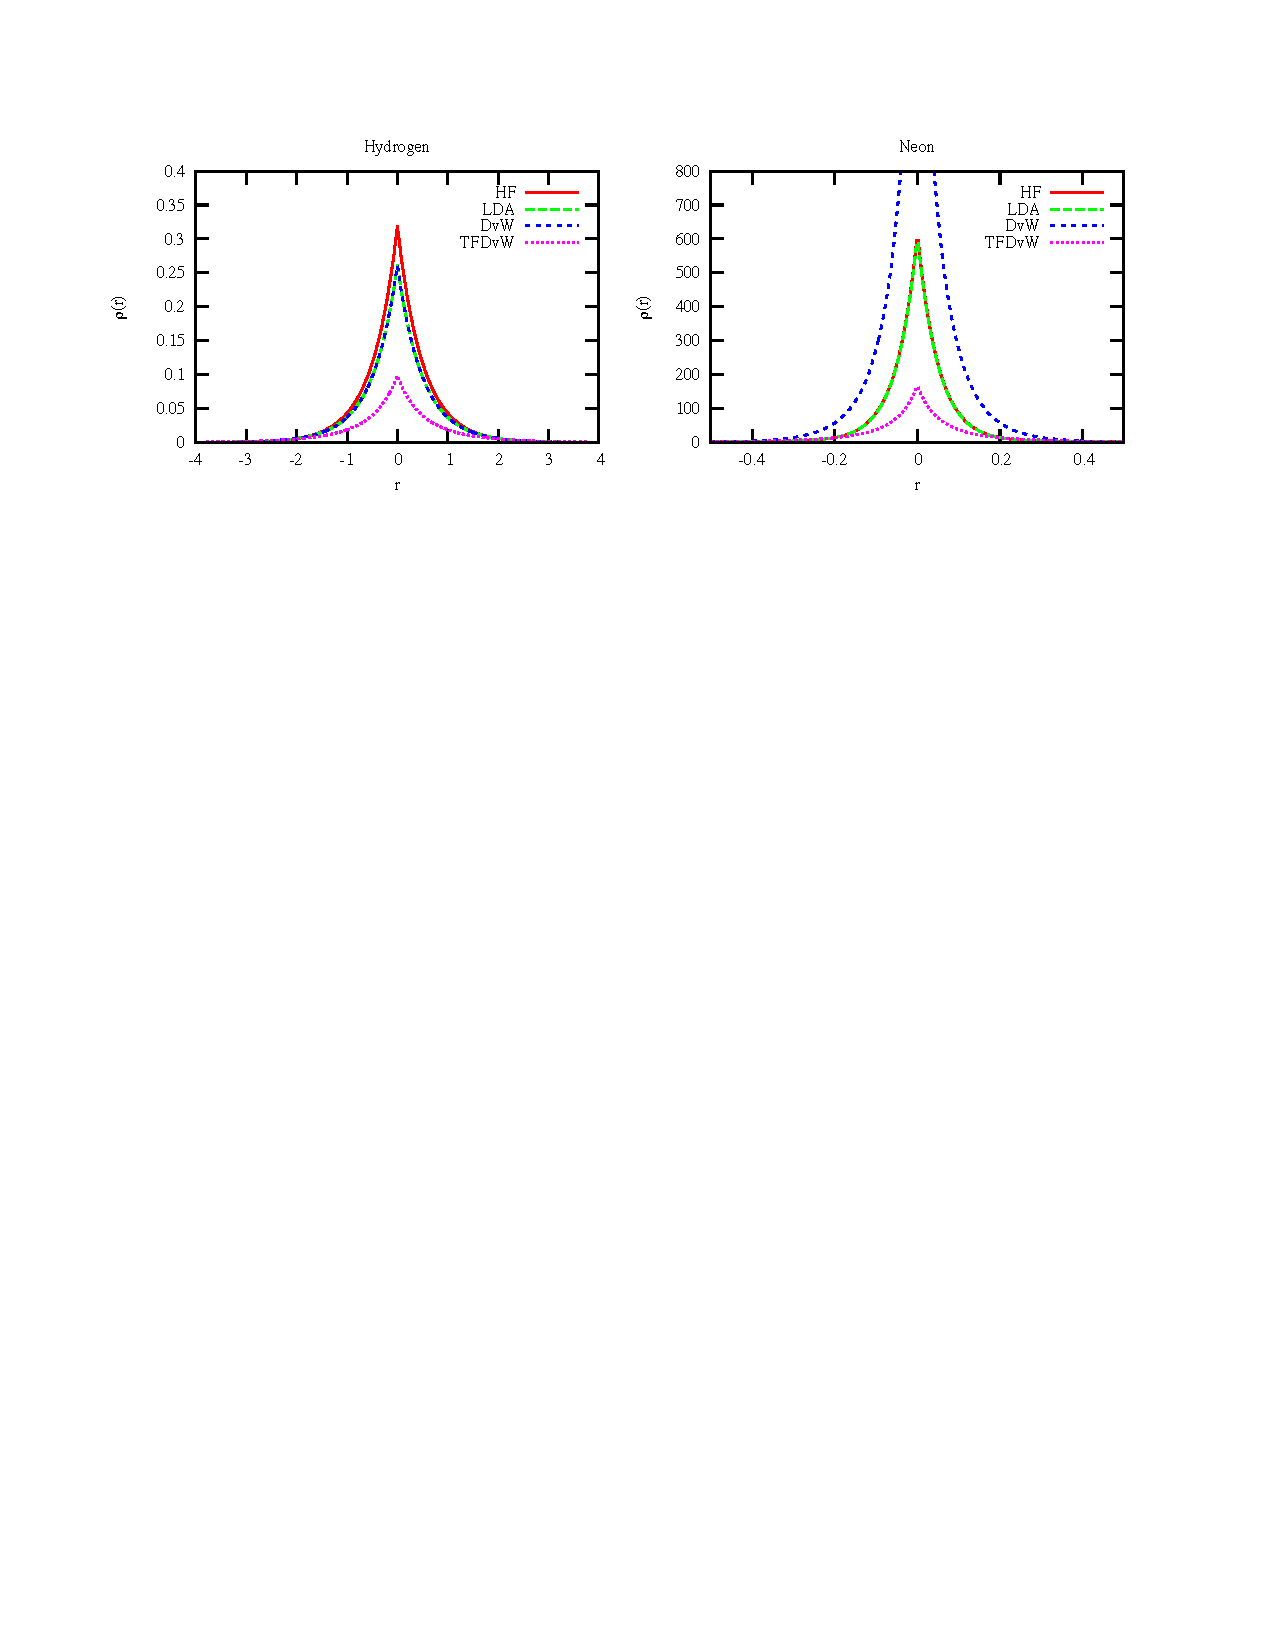
\includegraphics[scale=0.7, viewport = 50 560 550 755]{figures/of_atoms.pdf}
    \caption{\footnotesize{Density plots of hydrogen and neon atoms, calculated at different
	levels of theory.}}
    \label{fig:of-atoms}
\end{figure}

As can be seen from table \ref{tab:of-results}, we are able to reach self-consistent solutions that agree 
with previously reported numbers for small systems. All calculations were performed using a 9th order 
multiwavelet basis with an relative accuracy threshold of $\epsilon=10^{-6}$, and converged to a residual norm 
of $\|\orbital^{n+1}-\orbital^n\| < 10^{-6}$, which means that the presented numbers should be correct to
six significant digits. We observe, in accord with the claims of Chan and Karasiev, that the optimization is 
non-trivial, in particular when the Thomas-Fermi (TF) potential is included, and we were unable to reach convergence 
for bigger systems than the ones presented within a reasonable number of iterations. 

Without the TF potential, however, we observe similar convergence as for a single-orbital KS-DFT
calculation, and all the presented calculations reached the desired accuracy in about 10 iterations, starting 
from a random Gaussian density, but it seems that things get more complicated when more nuclear sites are 
introduced, as for instance the benzene molecule did not converge from a similar poor starting point. As already
mentioned, the inclusion of the purely repulsive TF term makes convergence much more problematic, and only the 
hydrogen atom converged straightforwardly. In all other calculations the TF term had to be introduced gradually.
By introducing a TF parameter $\alpha$ and writing the effective potential as
\begin{equation}
    v_{eff} = \alpha v_{\theta} + v_{nuc} + v_{el} + v_{xc}
\end{equation}
we were able to converge the many-electron systems in many intermediate steps, where for instance one could start 
with $\alpha=0.20$ and converge to $10^{-2}$, and then add five per cent TF ($\Delta\alpha=0.05$), converge again 
to $10^{-2}$, add another five per cent, and so on until the full TFDvW is reached. This, of course, requires a lot of 
iterations, and the bigger the system, the more sensitive it is to the TF potential, and consequently, a smaller 
$\Delta\alpha$ is required. Introduce the TF too fast, and the solution blows up and diverges. For instance, the neon 
energy was obtained using $\Delta\alpha=0.005$, and required more than 600 iterations. However, no attempt was made 
to optimize the parameters on this respect. 

\begin{figure}
    \centering
    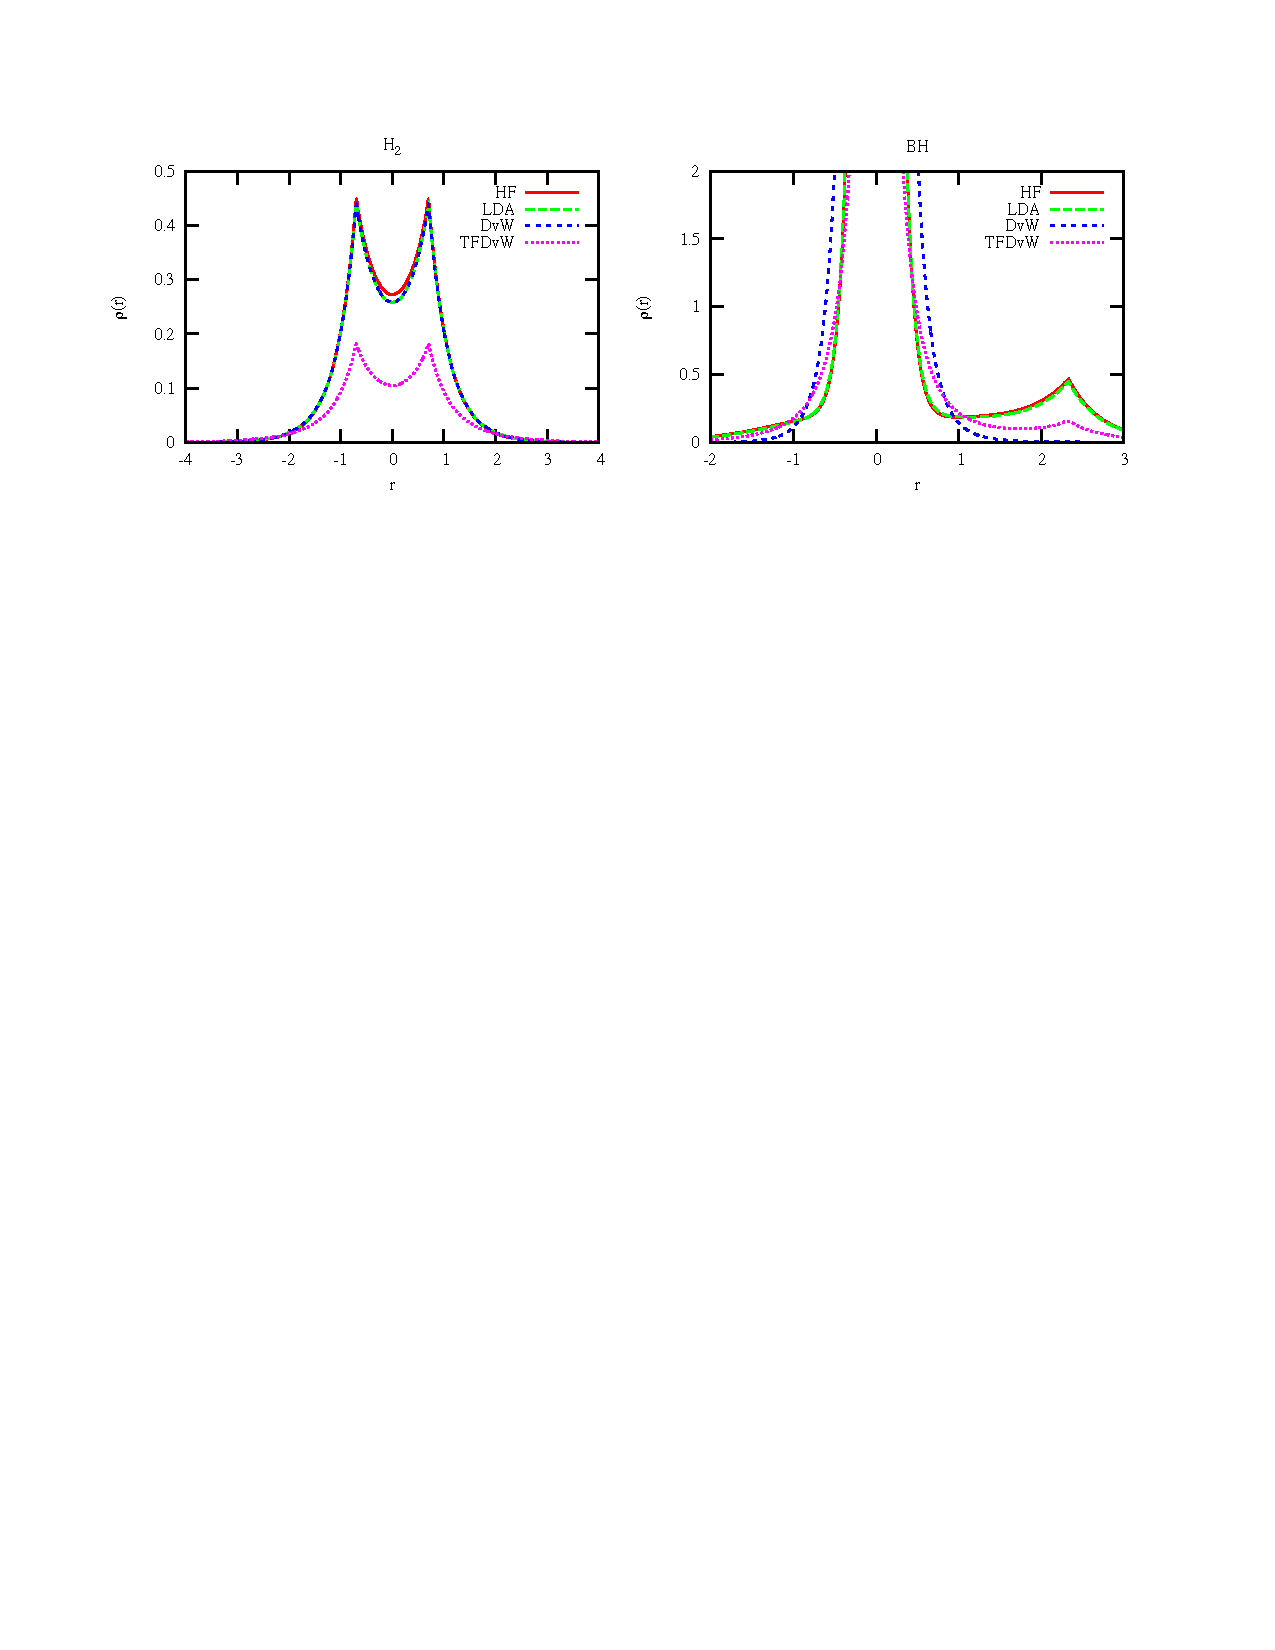
\includegraphics[scale=0.7, viewport = 50 560 550 755]{figures/of_molecules.pdf}
    \caption{\footnotesize{Density plots of $H_2$ and BH molecules, calculated at different
	levels of theory.}}
    \label{fig:of-molecules}
\end{figure}

If we examine the physics of these models we see that both DvW and TFDvW fail to reproduce the Hartree-Fock energies,
even qualitatively. As mentioned above, the von Weiz\"{a}cker functional is exact for one-orbital systems, which means
that DvW model is identical to LDA for the hydrogen and helium atoms, as well as the hydrogen molecule, as can be seen 
from the numbers. The same is observed in the density plots in figures \ref{fig:of-atoms} and \ref{fig:of-molecules},
where we can see the radial density of the hydrogen and neon atoms in fig. \ref{fig:of-atoms}, and the density along
the internuclear axis of the $H_2$ and $BH$ molecules in fig. \ref{fig:of-molecules}. 

From this we can conclude, as is already well established, that the Thomas-Fermi-Dirac-von-Weiz\"{a}cker models do
not perform well for atomic and molecular systems. It is common to introduce a parameter $\lambda$ for the von Weiz\"{a}cker
term in order to correct for a known over-estimation for molecular systems
\begin{equation}
    T_s = \lambda T_W + T_\theta
\end{equation}
and by adjusting this parameter one can get within a few per cent of the Hartree-Fock energy for the given atomic systems, 
as is shown by Chan \etal\cite{Chan:2000} using $\lambda=1/5$. However, this parameter is not universal, and the densities 
that are obtained are not equally accurate (see Ref.\cite{Chan:2000} for details).

\section{Outlook}
The purpose of this study was not to examine the performance of the given kinetic energy functionals on molecular
systems, as their inadequacies in this respect are well known, but rather to see whether the multiresolution framework
is appropriate for the solution of the OF-DFT Euler equation. It seems quite clear that its formulation as a one-orbital 
Kohn-Sham problem is not appropriate, as the convergence of the iterative solution for many-electron systems 
is problematic at best, as the Thomas-Fermi contribution had to be introduced very carefully to avoid divergence. However,
once the full TF potential had been included, high order convergence was not difficult to obtain, and accuracies of $10^{-9}$
was easily achieved.

Given the properties of the multiwavelet basis, which is easily parallelizable for the few global functions that are 
involved, and with representations that are free of basis set error, this could be the ideal framework for the development 
of better kinetic energy functionals, but this will require much more robust optimization algorithms. This will be subject
for further investigation.
